%%%%%%%%%%%%%%%%%%%%%%%%%%%%%%%%%%%%%%%%%%%%%%%
%%%This is a science homework template. Modify the preamble to suit your needs. 
%The junk text is   there for you to immediately see how the headers/footers look at first 
%typesetting.

\documentclass[12pt]{article}

%AMS-TeX packages
\usepackage{amssymb,amsmath,amsthm, mathtools} 
\usepackage{commath}
\usepackage[margin=1in]{geometry}
\usepackage{graphicx,ctable,booktabs}
\usepackage[retainorgcmds]{IEEEtrantools}
\usepackage{cancel}
\usepackage{wrapfig}
\usepackage{braket}
\usepackage{enumitem}
\usepackage{pdfpages}
\usepackage{subcaption}
\usepackage{xurl}

\usepackage{graphicx}
\usepackage{subfig}

%Redefining sections as problems

\makeatletter
\newenvironment{problem}{\@startsection
	{section}
	{1}
	{-.2em}
	{-3.5ex plus -1ex minus -.2ex}
	{2.3ex plus .2ex}
	{\pagebreak[3]%forces pagebreak when space is small; use \eject for better results
		\large\bf\noindent{Problem }
	}
}
{%\vspace{1ex}\begin{center} \rule{0.3\linewidth}{.3pt}\end{center}}
	\begin{center}\large\bf \ldots\ldots\ldots\end{center}}
\makeatother

%Fancy-header package to modify header/page numbering 

\usepackage{fancyhdr}
\pagestyle{fancy}
\lhead{Problem \thesection}
\chead{} 
\rhead{\thepage} 
\lfoot{\small\scshape PHYS 600} 
\cfoot{} 
\rfoot{\footnotesize HW 5} 
\renewcommand{\headrulewidth}{.3pt} 
\renewcommand{\footrulewidth}{.3pt}
\setlength\voffset{-0.25in}
\setlength\textheight{648pt}
\allowdisplaybreaks

\newcommand{\partder}[3]{\ensuremath{\left(\frac{\partial {#1}}{\partial {#2}}\right)_{#3}}}

\newcommand{\braks}[1]{\ensuremath{\left\langle{#1} \right\rangle} }

\newcommand{\Omx}[1]{\ensuremath{\Omega_\mathrm{#1} } }
\newcommand{\rhox}[1]{\ensuremath{\rho_\mathrm{#1} } }

\setlength{\parindent}{0pt} % No indent by default

%%%%%%%%%%%%%%%%%%%%%%%%%%%%%%%%%%%%%%%%%%%%%%%

%
%Contents of problem set
%    

\begin{document}
	
	\title{PHYS 600: Homework 5}
	\author{Yarone Tokayer}
	\date{December 3, 2023}
	
	\maketitle
	
	\thispagestyle{empty}
	
	%			\begin{figure}
		%				\centering
		%				\fbox{
			%					\begin{minipage}{\linewidth}
				%						\centering
				%						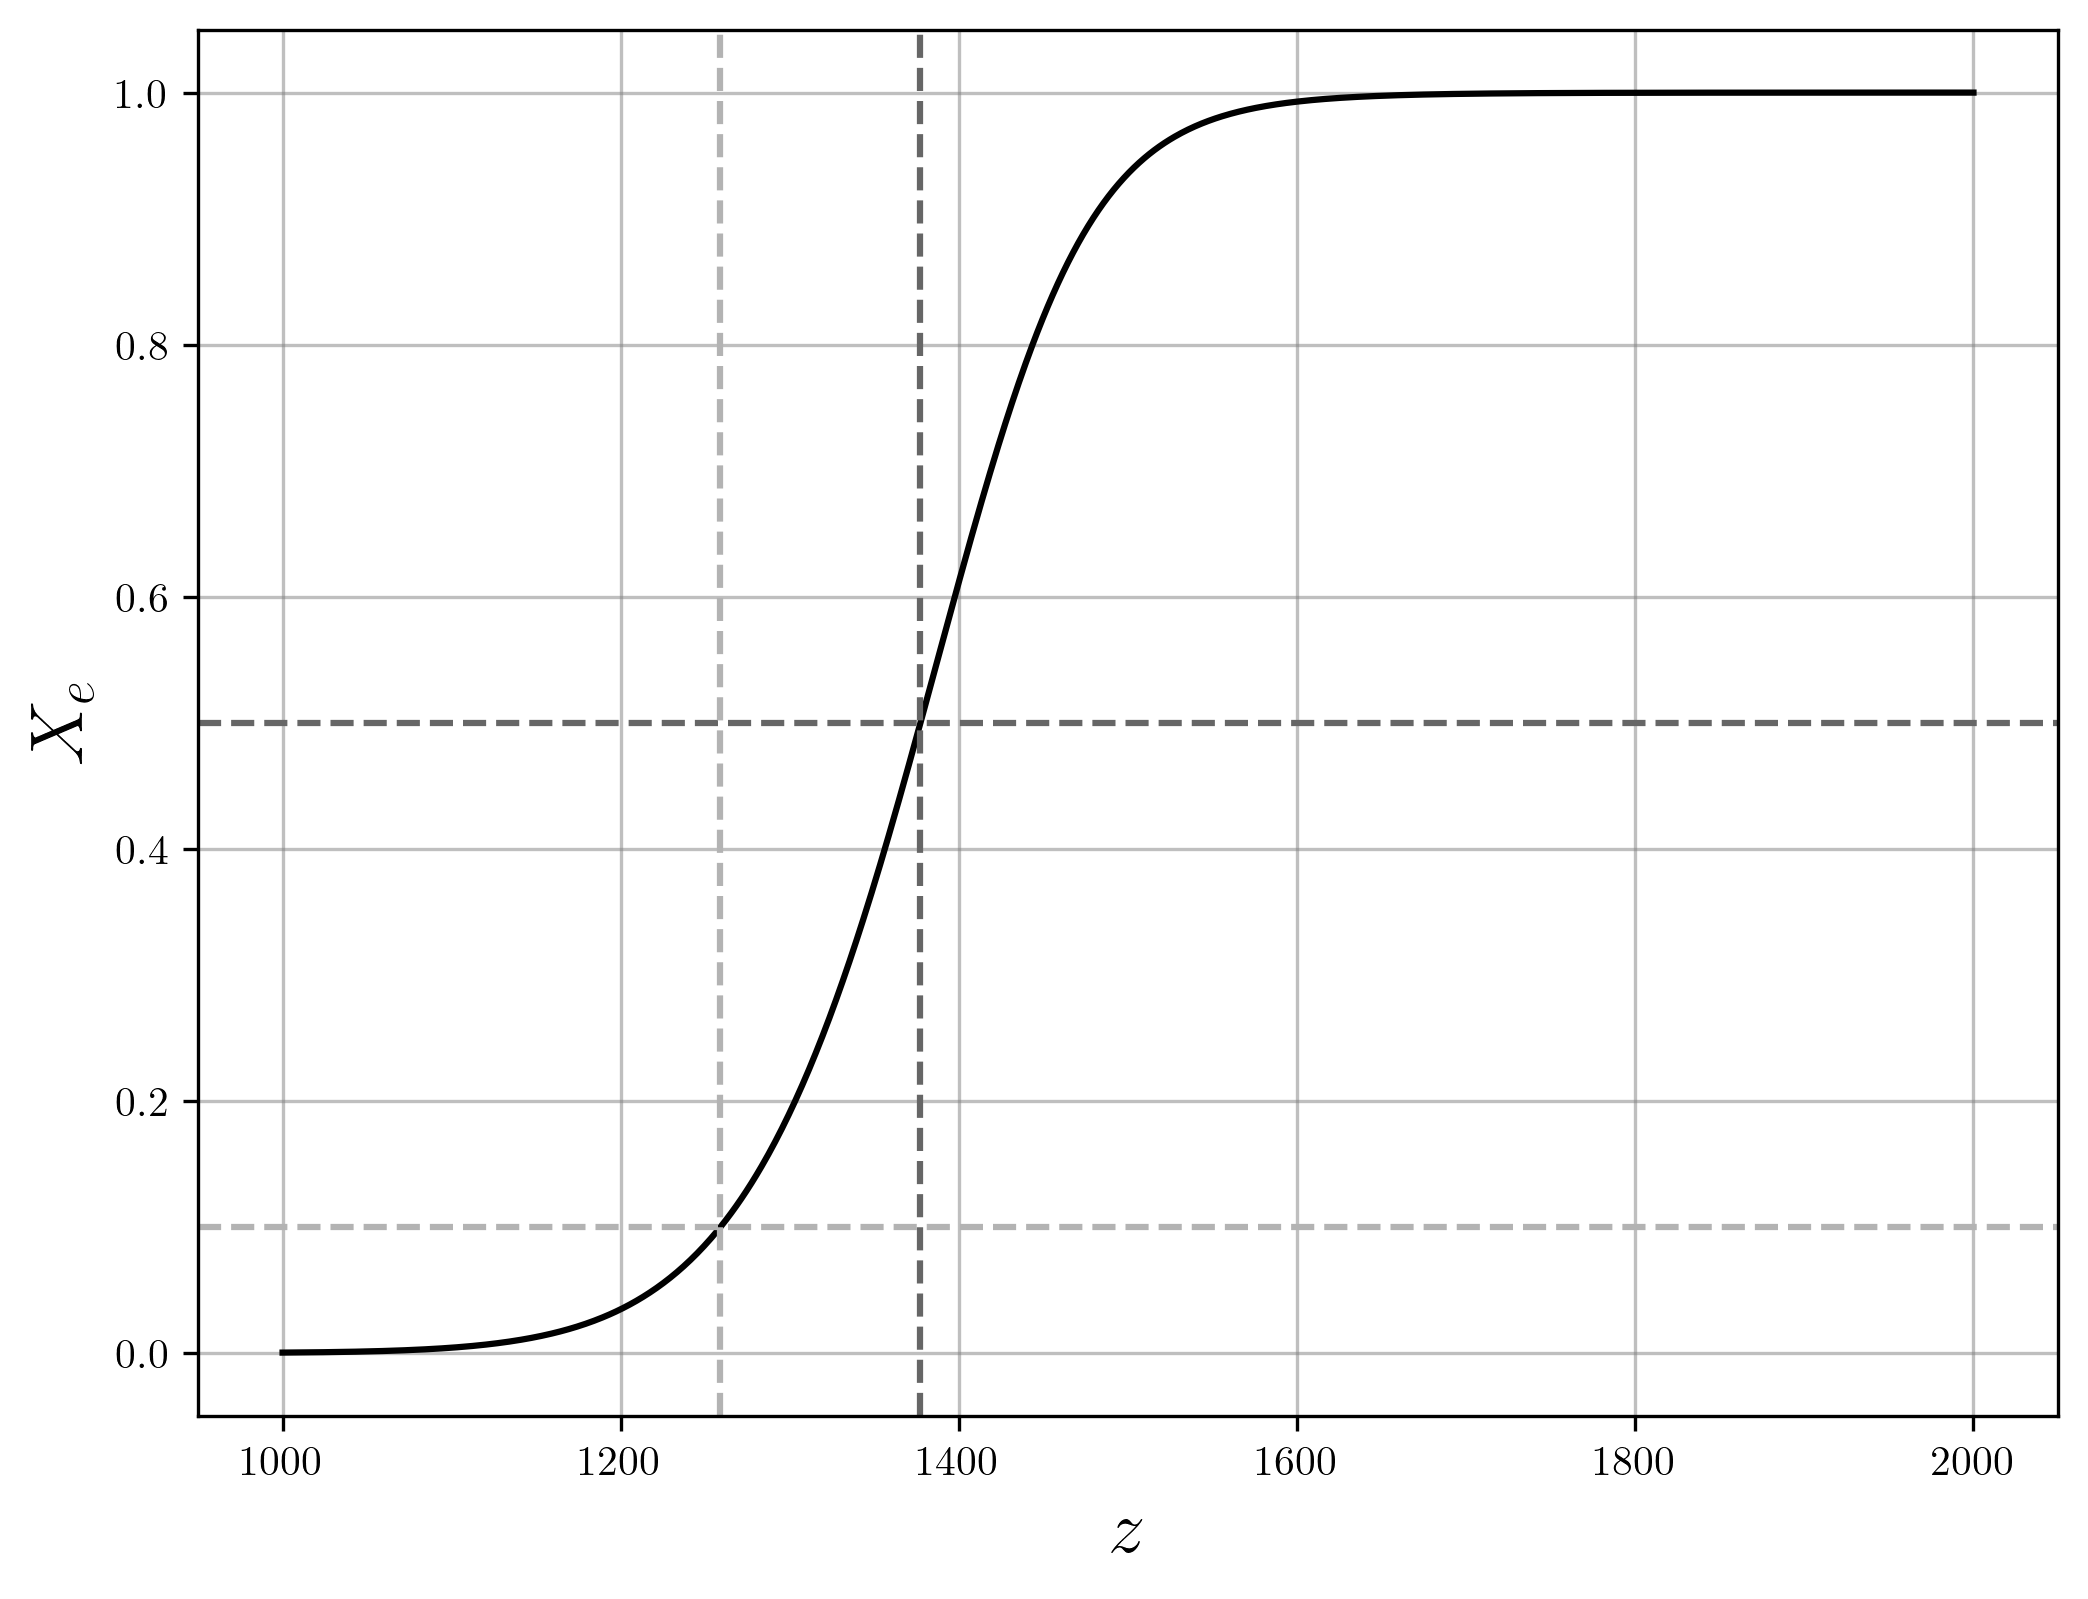
\includegraphics[width=0.65\linewidth]{x_e_plot.png}
				%						\caption{The free electron fraction as a function of redshift around the epoch of reionization.  The redshifts at which $X_e$ = 0.1 and 0.5 are indicated.}\label{fig:x_e}
				%					\end{minipage}
			%				}
		%			\end{figure}

	\begin{problem}{Growth of Matter Perturbations---Matter and Radiation}
		\begin{itemize}
			\item 
			
			\item 
			
			\item
			
			\item 
			
			\item 

		\end{itemize} 
	\end{problem}
	
	\begin{problem}{Spherical Collapse}
		The equation of motion for a single shell enclosing a mass of $M$ during spherical collapse is \begin{align*}
			\frac{\dif^2 r}{\dif t^2} &= -\frac{GM}{r}
			\\
			\implies \frac{1}{2}\left(\frac{\dif r}{\dif t}\right)^2 - \frac{GM}{r} &= E
			\\
			\frac{1}{2}\left(\frac{\dif r}{\dif \theta}\frac{1}{\dif t/\dif\theta}\right)^2 - \frac{GM}{r} &= E
			\\
			\frac{1}{2}\left(\frac{A\sin\theta}{B(1-\cos\theta)}\right)^2 - \frac{GM}{A(1-\cos\theta)} &= E
			\\
			\frac{GM}{2A}\left(\frac{\sin\theta}{1-\cos\theta}\right)^2 - \frac{2\abs{E}}{1-\cos\theta} &= E
			\\
			\frac{GM}{2A}\frac{1-\cos^2\theta}{(1-\cos\theta)^2} - \frac{2\abs{E}}{1-\cos\theta} &= E
			\\
			\frac{1+\cos\theta}{1-\cos\theta}\abs{E} - \frac{2\abs{E}}{1-\cos\theta} &= E
			\\
			\frac{-\abs{E}+\abs{E}\cos\theta}{1-\cos\theta} &= E
			\\
			-\abs{E} &= E
		\end{align*} We have shown that this is a parametric solution for $E<0$, as desired.
	\end{problem}
	
	\begin{problem}{Equality Scale}
		
	\end{problem}
	
	\begin{problem}{A Study in Simulations}
		
		\begin{description}
			\item[Orienting Yourself : The Linear Power Spectrum] description
			
			\item[Non-linear Power Spectrum and Structure Growth] description
			
			\item[Computing the Growth Function] description
			
			\item[Halo Mass Function] description
		\end{description}
	
	\end{problem}


% Appendix
\appendix
\section{Python code}
%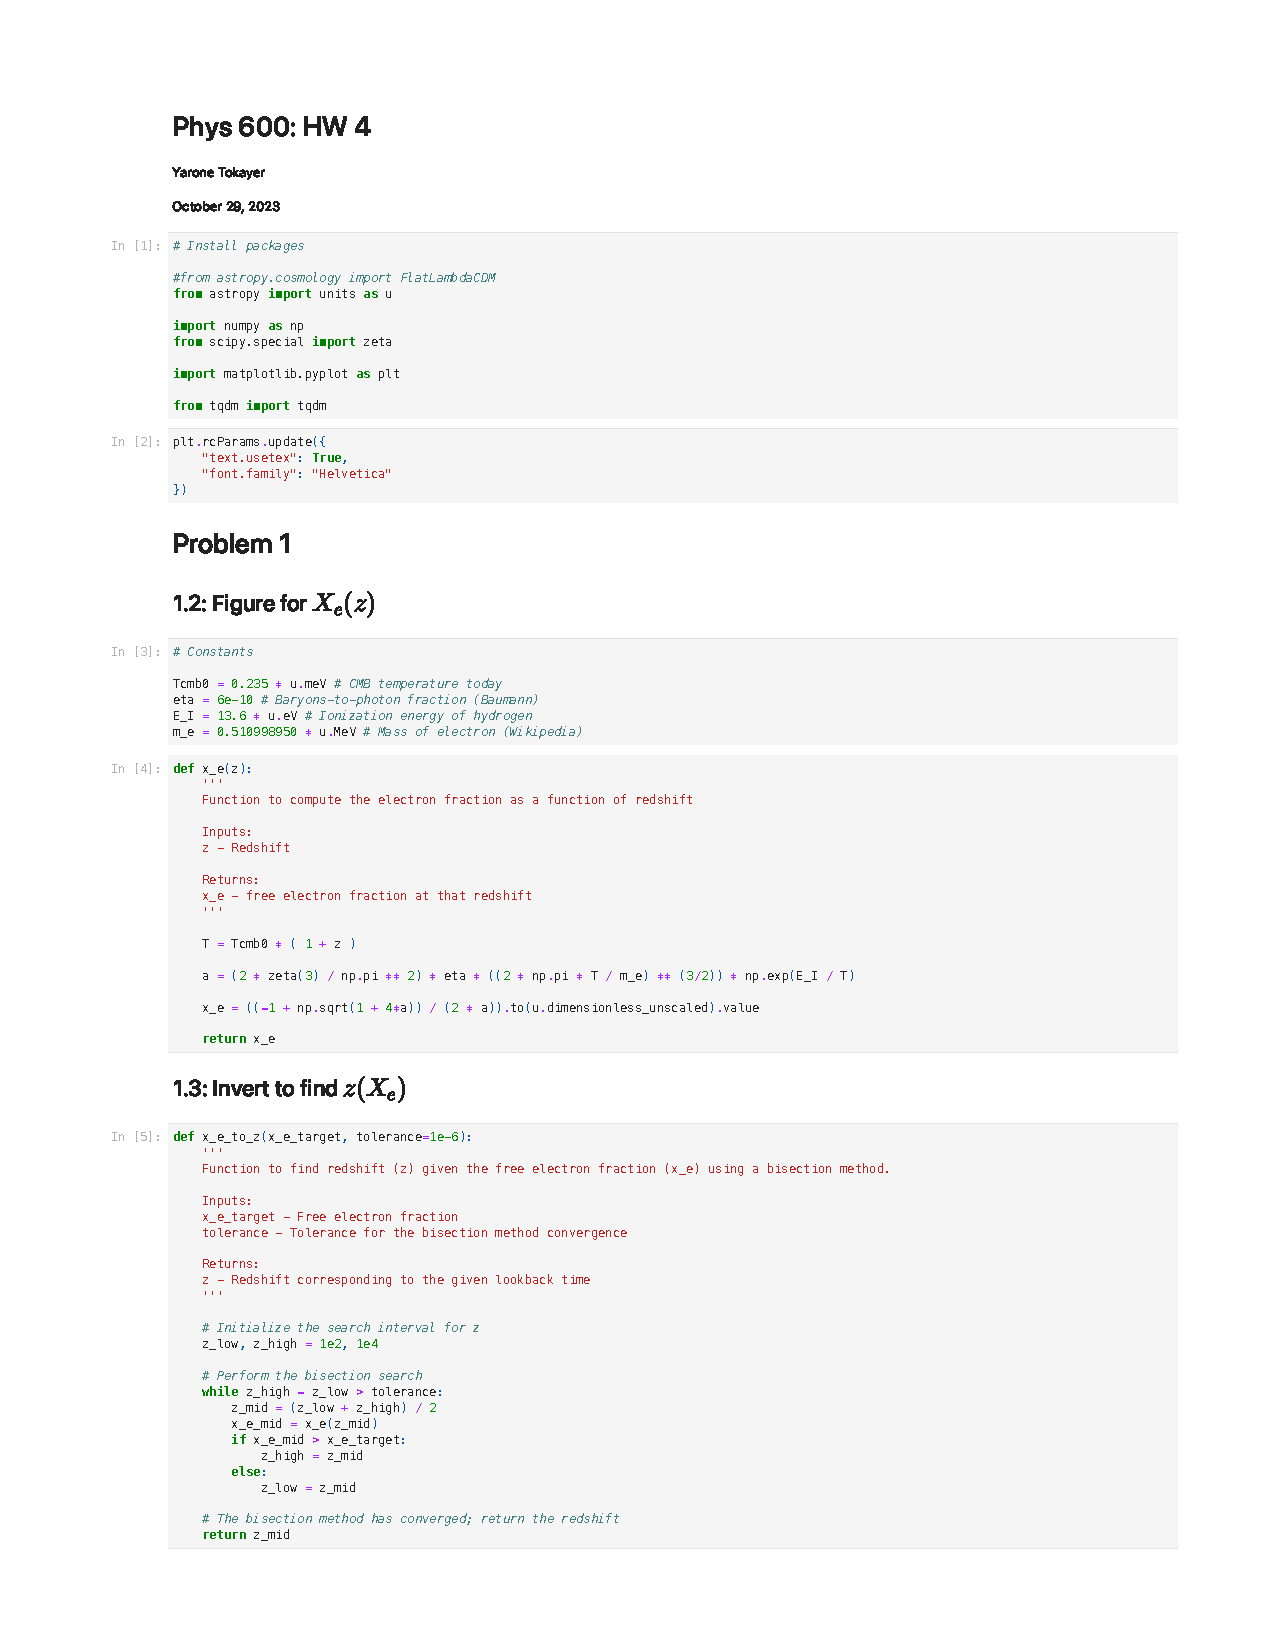
\includepdf[pages=-, frame=true, scale=0.9]{/Users/yaronetokayer/Yale Drive/Classes/PHYS 600/phys600 hw/phys600 hw 4/phys600 hw 4 work.pdf}



\end{document}